%Predicates
%	Vis dem alle
%		Men snak kun om de seje
%		Func dep
%		Referential integrity
%		Compare
%	Vis kode for dem
%Hvorfor er de nyttige og hvordan løser de vores problem
%Hvordan anvendes de
%Alternativ implementering/design
%Andre nyttige predicates - Har vi covered enough

\section{Predicates}
\begin{frame}{Predicates}{Agenda}
  \begin{itemize}
    \item<1-> Why are they useful?
    \item<1-> Usage/Implementation 
    \item<1-> Alternative Forms of Implementation
  \end{itemize}
\end{frame}
%%%%%%%%%%%%%%%%

\subsection{Why are they useful?}
\begin{frame}{Predicates}{Why are they useful?}
	\begin{itemize}
		\item<1-> Systems level testing
			\begin{itemize}
				\item Data loss
			\end{itemize}
		\item<2-> Source to target test
		\item<2-> 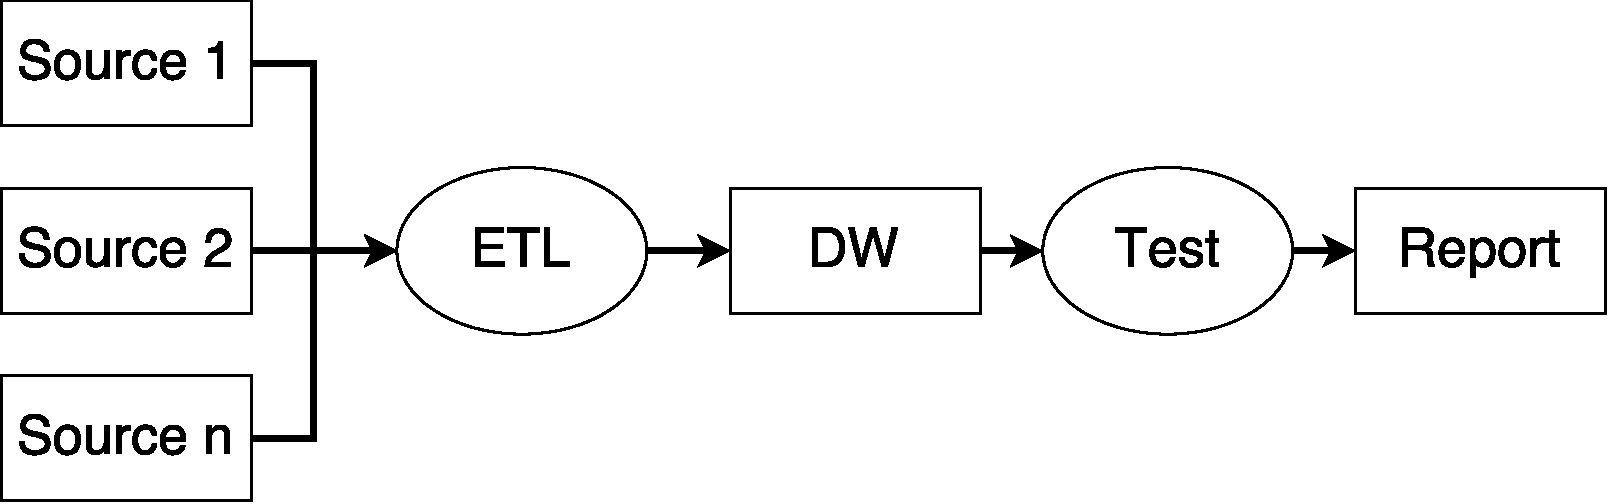
\includegraphics[width=8.5cm]{figures/scenario.pdf}
		\item<3-> Regression testing
		\item<3-> Business Rules
	\end{itemize}
\end{frame}

\begin{frame}{Predicates}{Why are they useful?}
	\begin{block}{Predicates available in SKiRaff}
		\begin{itemize}
			\item<1-> RowCountPredicate
			\item<1-> ColumnNotNullPredicate
			\item<1-> ReferentialIntegrityPredicate
			\item<1-> FunctionalDependencyPredicate
			\item<1-> SCDVersionPredicate
			\item<1-> CompareTablePredicate
			\item<1-> RuleRowPredicate
			\item<1-> RuleColumnPredicate
		\end{itemize}
	\end{block}
\end{frame}

\begin{frame}{Predicates}{Why are they useful?}
	\begin{block}{Predicates available in SKiRaff}
		\begin{itemize}
			\item<1-> RowCountPredicate
			\item<1-> ColumnNotNullPredicate
			\item<1-> \textbf{ReferentialIntegrityPredicate}
			\item<1-> \textbf{FunctionalDependencyPredicate}
			\item<1-> SCDVersionPredicate
			\item<1-> CompareTablePredicate
			\item<1-> \textbf{RuleRowPredicate}
			\item<1-> RuleColumnPredicate
		\end{itemize}
	\end{block}
\end{frame}

\subsection{Usage/Implementation }
\begin{frame}{Predicates}{Usage - Functional Dependency}
	\begin{block}{Functional Dependency - Why is it useful?}
		\begin{itemize}
			\item<1-> A, B --> C
			\item<2-> DW holds certain hierarchical properties
		\end{itemize}
	\end{block}
\end{frame}

\begin{frame}{Predicates}{Usage - Functional Dependency}
	\begin{block}{Setup:}
		\insertcodefile{FunctionalDependencyPredicate.py}{}
	\end{block}
	\begin{block}{SQL querie:}
		\insertcodefileSQL{SQLFunctionalDependency.sql}{}
	\end{block}
\end{frame}

\begin{frame}{Predicates}{Implementation - Functional Dependency}
	\insertcodefile{funDep1.py}{}
\end{frame}

\begin{frame}{Predicates}{Implementation - Functional Dependency}
	\insertcodefile{funDep2.py}{}
	\begin{block}{SQL querie:}
		\insertcodefileSQL{SQLFunctionalDependency.sql}{}
	\end{block}
\end{frame}

\begin{frame}{Predicates}{Implementation - Functional Dependency}
	\insertcodefile{funDep3.py}{}
\end{frame}

\begin{frame}{Predicates}{Usage - Referential Integrity}
	\begin{block}{Referential Integrity - Why is it useful?}
		\begin{itemize}
			\item<1-> Most DBMS's have various referential integrity rules
			\item<2-> Not removing the correct data from all tables
		\end{itemize}
	\end{block}
\end{frame}

\begin{frame}{Predicates}{Usage - Referential Integrity}
  \begin{block}{Setup:}
		\insertcodefile{ReferentialIntegrityPredicate.py}{}
	\end{block}
	\begin{block}{SQL querie:}
		\insertcodefileSQL{SQLReferentialIntegrityPredicate.sql}{}
	\end{block}
\end{frame}

\begin{frame}{Predicates}{Implementation - Referential Integrity}
	\insertcodefile{ref1.py}{}
\end{frame}

\begin{frame}{Predicates}{Implementation - Referential Integrity}
	\insertcodefile{ref2.py}{}
\end{frame}

\begin{frame}{Predicates}{Implementation - Referential Integrity}
	\insertcodefile{ref3.py}{}
\end{frame}

\begin{frame}{Predicates}{Implementation - Referential Integrity}
	\insertcodefile{ref4.py}{}
\end{frame}

\begin{frame}{Predicates}{Usage - RuleRowPredicate}
	\begin{block}{RuleRowPredicate - Why is it useful?}
		\begin{itemize}
			\item<1-> Gives the user freedom to check for things our other predicate can't
			\item<1-> But with an easy setup
			\item<2-> However slower than others due to the lack of SQL implementation
		\end{itemize}
	\end{block}
\end{frame}

\begin{frame}{Predicates}{Usage - RuleRowPredicate}
  \begin{block}{Setup:}
		\insertcodefile{RuleRowPredicate.py}{}
	\end{block}
\end{frame}

\begin{frame}{Predicates}{Implementation - RuleRowPredicate}
		\insertcodefile{ruleRow1.py}{}
\end{frame}

\begin{frame}{Predicates}{Implementation - RuleRowPredicate}
		\insertcodefile{ruleRow2.py}{}
\end{frame}

\subsection{Alternative Implementation}
\begin{frame}{Predicates}{Alternative Implementation - row\_count\_predicate}
	\begin{block}{Now: SQL queries}
		\insertcodefileline{row_count_predicate_new.py}{}{25}{36}
	\end{block}
\end{frame}

\begin{frame}{Predicates}{Alternative Implementation - row\_count\_predicate}
	\begin{block}{Alternative: Representation objects in python}
		\insertcodefileline{row_count_predicate_old.py}{}{21}{32}
	\end{block}
\end{frame}

	
